The aim of this project is to analyze a dataset collected from NBA Rookies' games. This set contains 1340 samples, each one described by the 21 features listed below: 
\begin{itemize}
	\item Name of the player (Name): string;
	\item Number of games played (GP): discrete variable;
	\item Minutes played per game (MIN): continuous variable;
	\item Points scored per game (PTS): continuous variable;
	\item Field goals made per game (FGM): continuous variable;
	\item Field goals attempts per game (FGA): continuous variable;
	\item Field goals percent per game (FG\%): continuous variable;
	\item Three point shots made per game (3P MADE): continuous variable;
	\item Three points shots attempts per game (3PA): continuous variable;
	\item Three point shots attempts per game (3P\%): continuous variable;
	\item Free throws made per game (FTM): continuous variable;
	\item Free throws attempts per game (FTA): continuous variable;
	\item Free throws made per game (FT\%): continuous variable;
	\item Number of offensive rebounds per game (OREB): continuous variable;
	\item Number of defensive rebounds per game (DREB): continuous variable;
	\item Number of rebounds per game (REB): continuous variable;
	\item Number of assists per game (AST): continuous variable;
	\item Number of steals per game (STL): continuous variable;
	\item Number of blocks per game (BLK): continuous variable;
	\item Number of turnovers per game (TOV): continuous variable;
	\item Output variable (TARGET\_5Yrs): 1 if career duration $\geq 5$, 0 otherwise\\
\end{itemize} 

The histograms of the 19 useful regressors are shown in \Fig~\ref{fig:Histograms}.
\begin{figure}[H]
	\centering
	\begin{subfigure}{.3\textwidth}
		\centering
		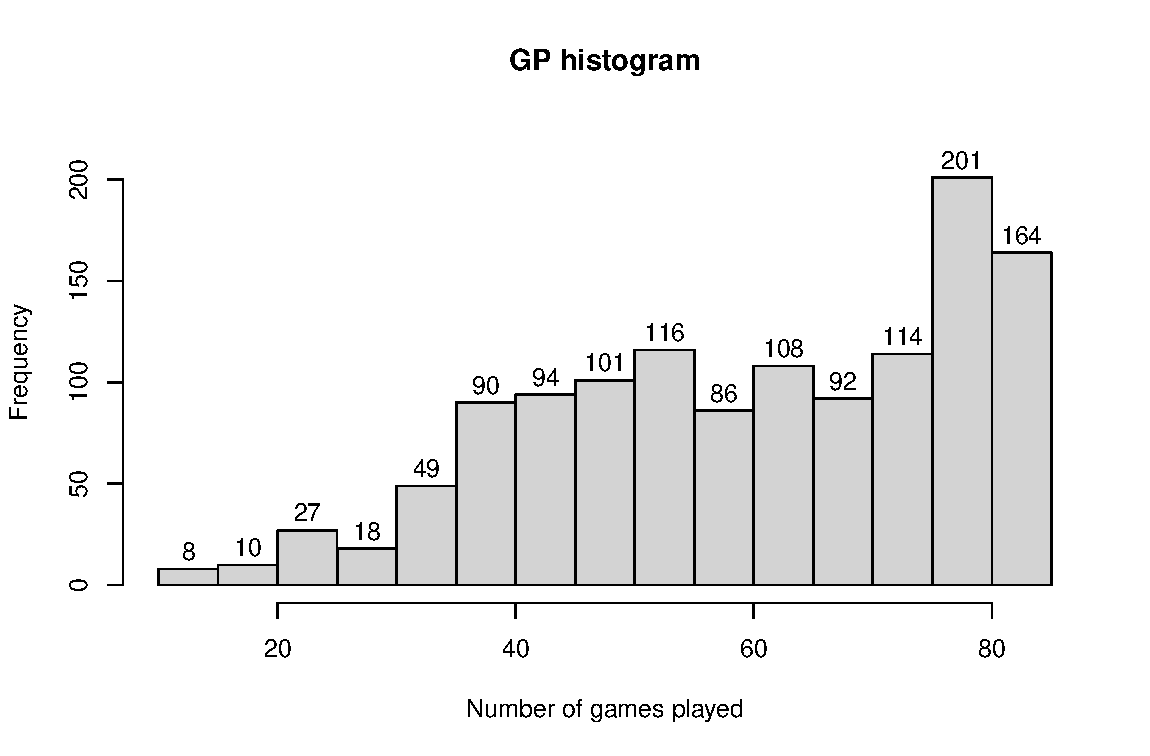
\includegraphics[width=0.5\linewidth]{ImageFiles/Histograms/histogram_gp}
		\caption{}
		\label{fig:HistGP}
	\end{subfigure}%
	\begin{subfigure}{.3\textwidth}
		\centering
		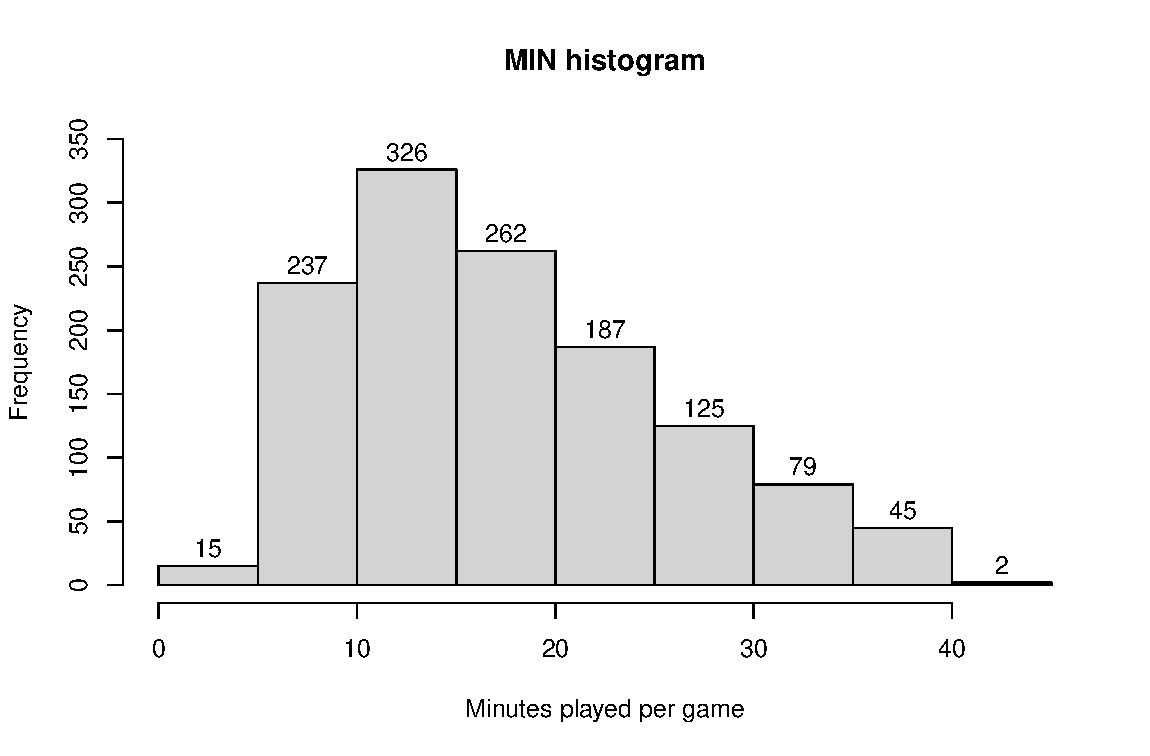
\includegraphics[width=0.5\linewidth]{ImageFiles/Histograms/histogram_min}
		\caption{}
		\label{fig:HistMIN}
	\end{subfigure}%
	\begin{subfigure}{.3\textwidth}
		\centering
		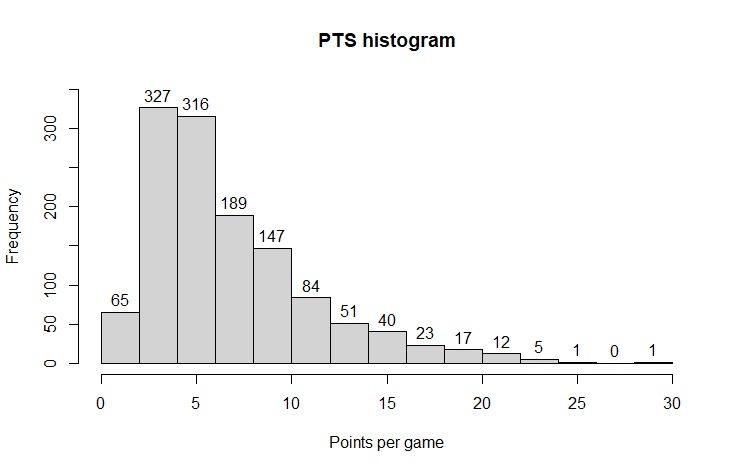
\includegraphics[width=0.5\linewidth]{ImageFiles/Histograms/histogram_pts}
		\caption{}
		\label{fig:HistPTS}
	\end{subfigure}
	\begin{subfigure}{.3\textwidth}
		\centering
		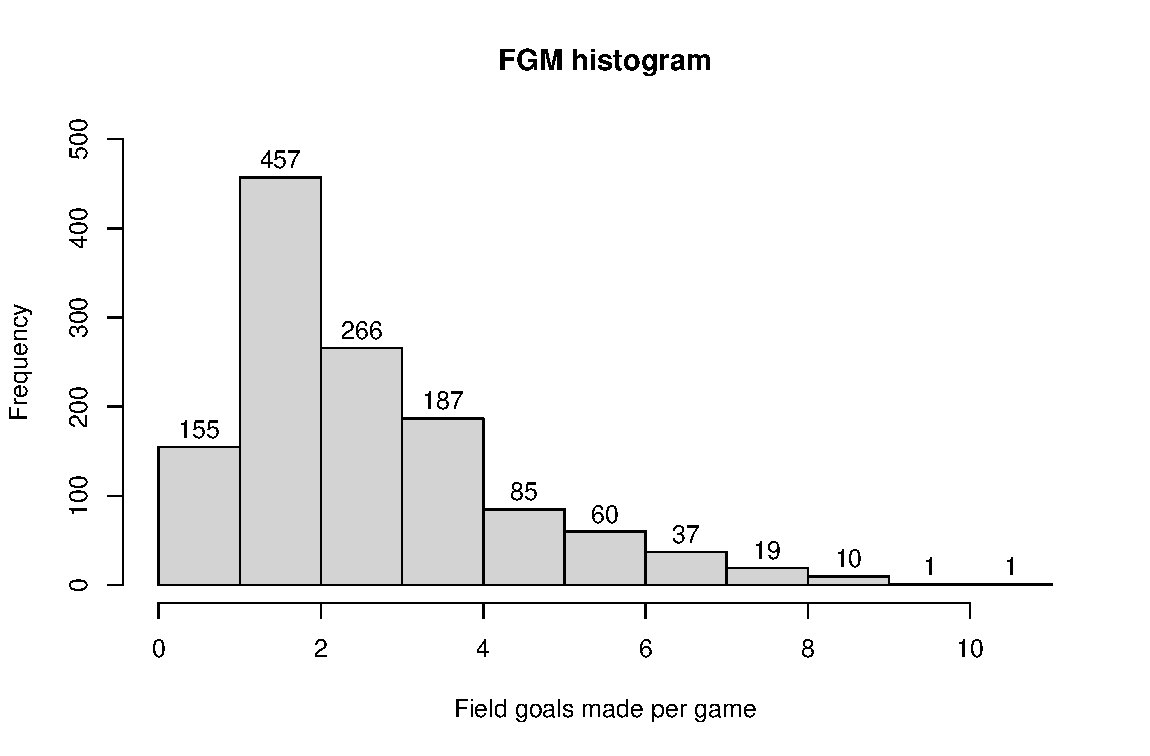
\includegraphics[width=0.5\linewidth]{ImageFiles/Histograms/histogram_fgm}
		\caption{}
		\label{fig:HistFGM}
	\end{subfigure}%
	\begin{subfigure}{.3\textwidth}
		\centering
		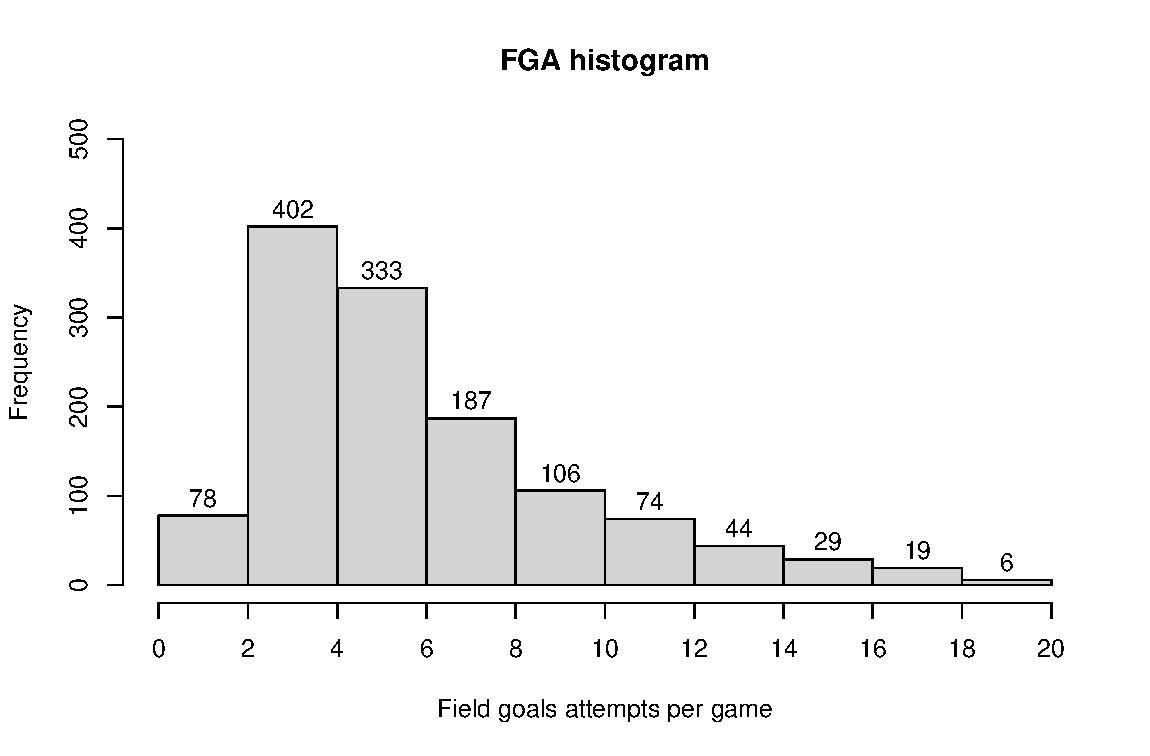
\includegraphics[width=0.5\linewidth]{ImageFiles/Histograms/histogram_fga}
		\caption{}
		\label{fig:HistFGA}
	\end{subfigure}%
	\begin{subfigure}{.3\textwidth}
		\centering
		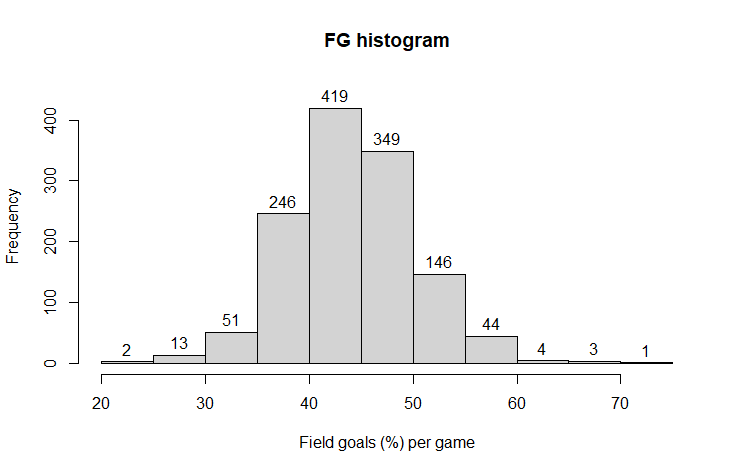
\includegraphics[width=0.5\linewidth]{ImageFiles/Histograms/histogram_fg}
		\caption{}
		\label{fig:HistFG}
	\end{subfigure}
	\begin{subfigure}{.3\textwidth}
		\centering
		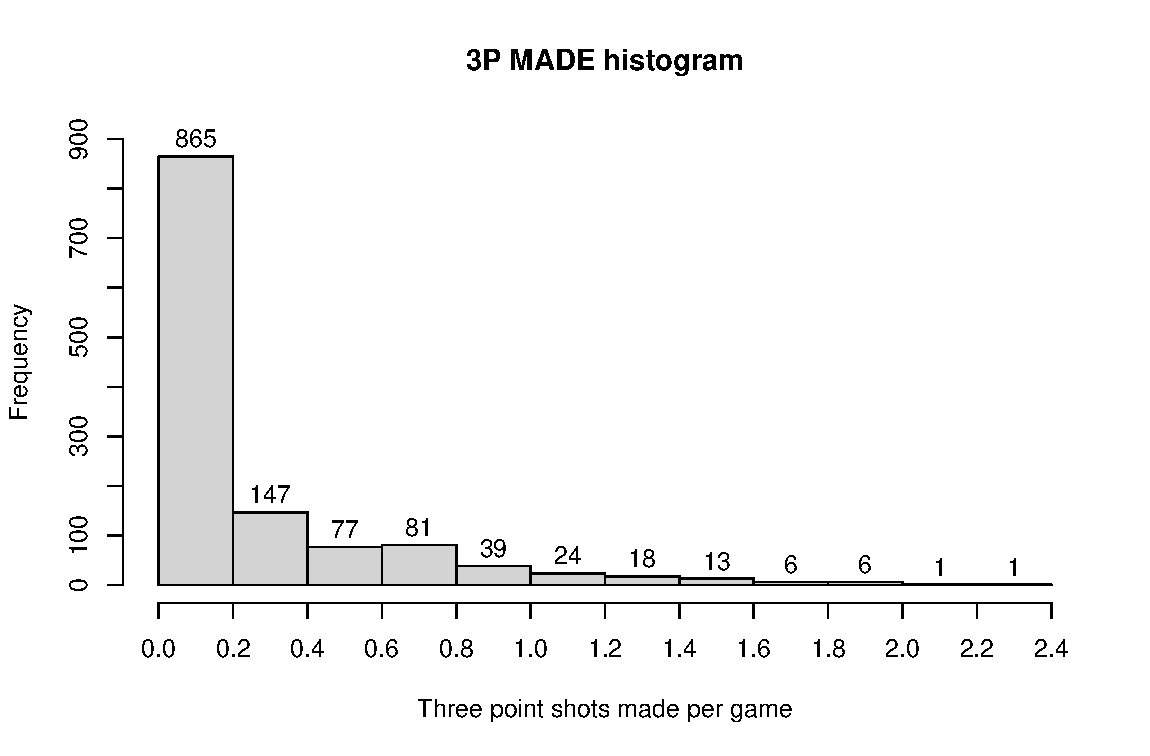
\includegraphics[width=0.5\linewidth]{ImageFiles/Histograms/histogram_x3pmade}
		\caption{}
		\label{fig:HistX3PMADE}
	\end{subfigure}%
	\begin{subfigure}{.3\textwidth}
		\centering
		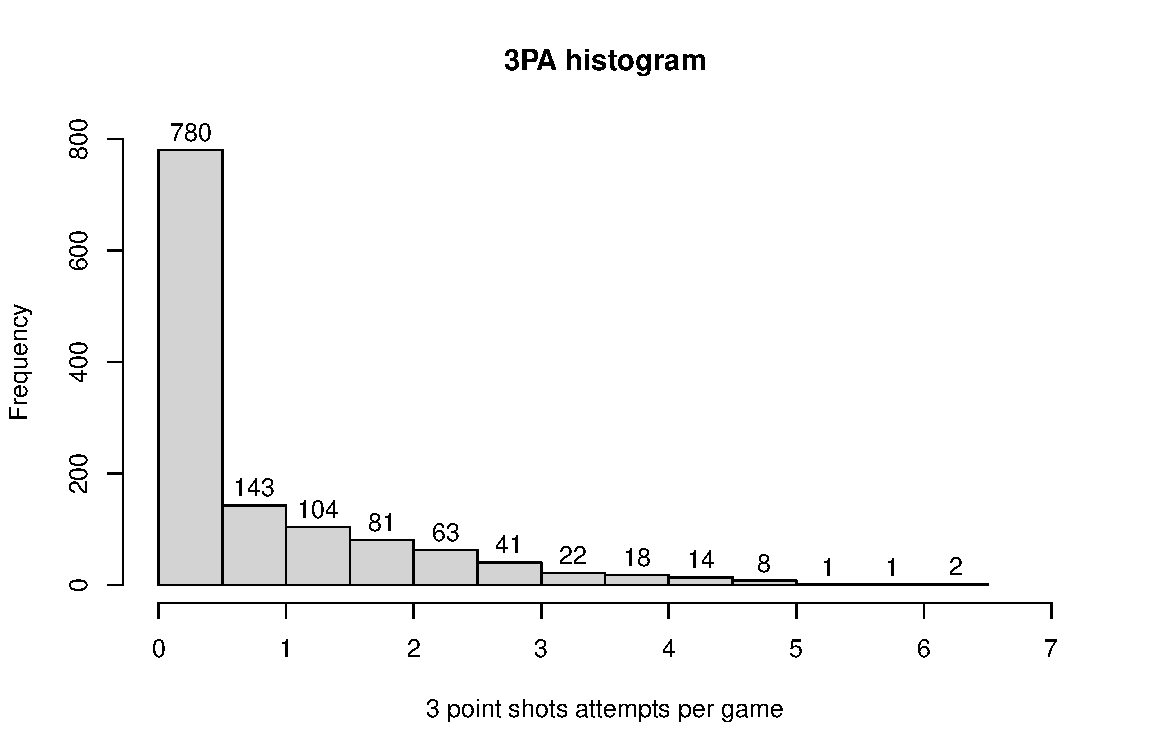
\includegraphics[width=0.5\linewidth]{ImageFiles/Histograms/histogram_x3pa}
		\caption{}
		\label{fig:HistX3PA}
	\end{subfigure}%
	\begin{subfigure}{.3\textwidth}
		\centering
		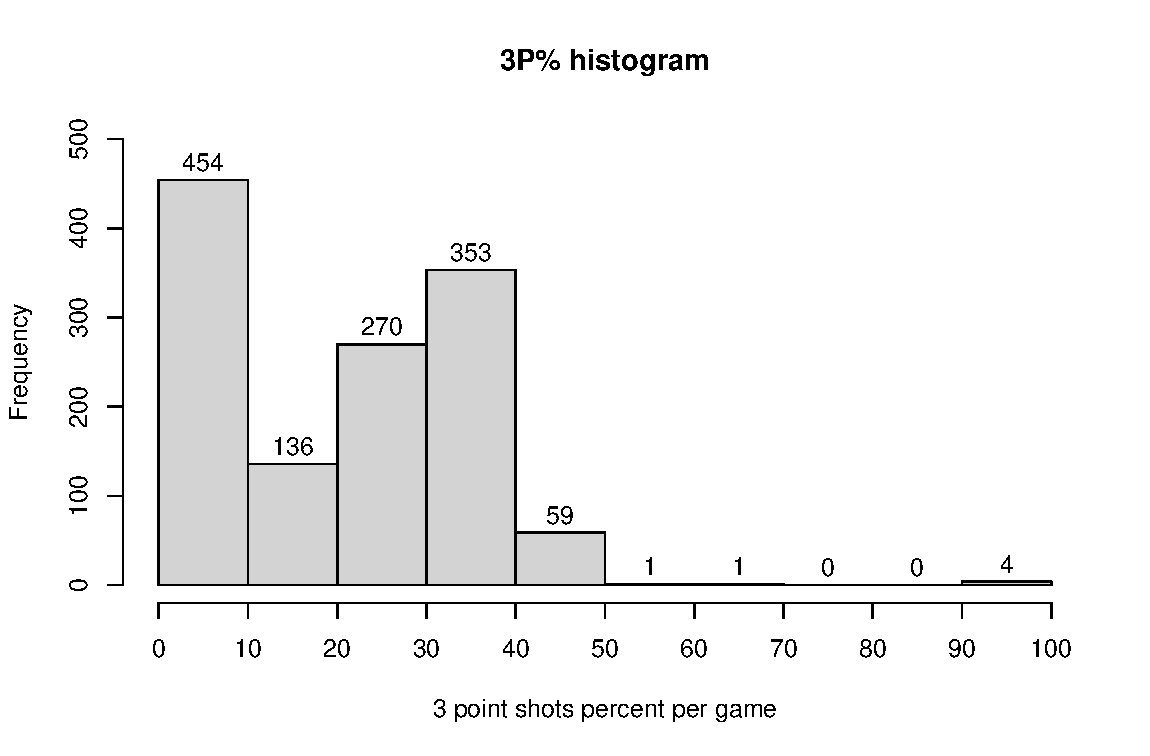
\includegraphics[width=0.5\linewidth]{ImageFiles/Histograms/histogram_x3p}
		\caption{}
		\label{fig:HistX3P}
	\end{subfigure}
	\begin{subfigure}{.3\textwidth}
		\centering
		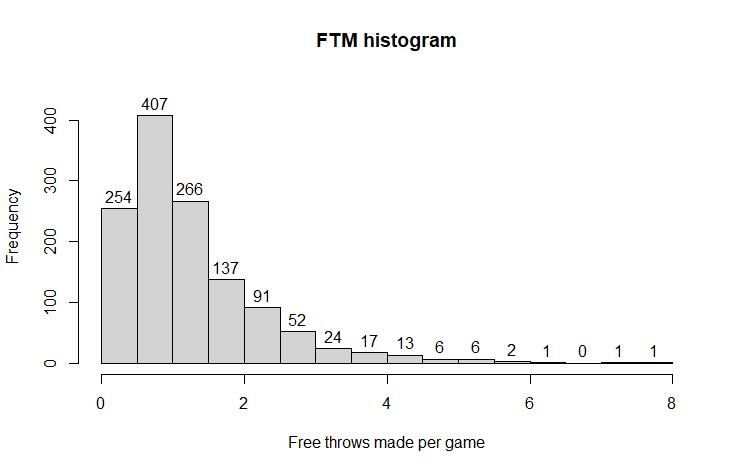
\includegraphics[width=0.5\linewidth]{ImageFiles/Histograms/histogram_ftm}
		\caption{}
		\label{fig:HistFTM}
	\end{subfigure}%
	\begin{subfigure}{.3\textwidth}
		\centering
		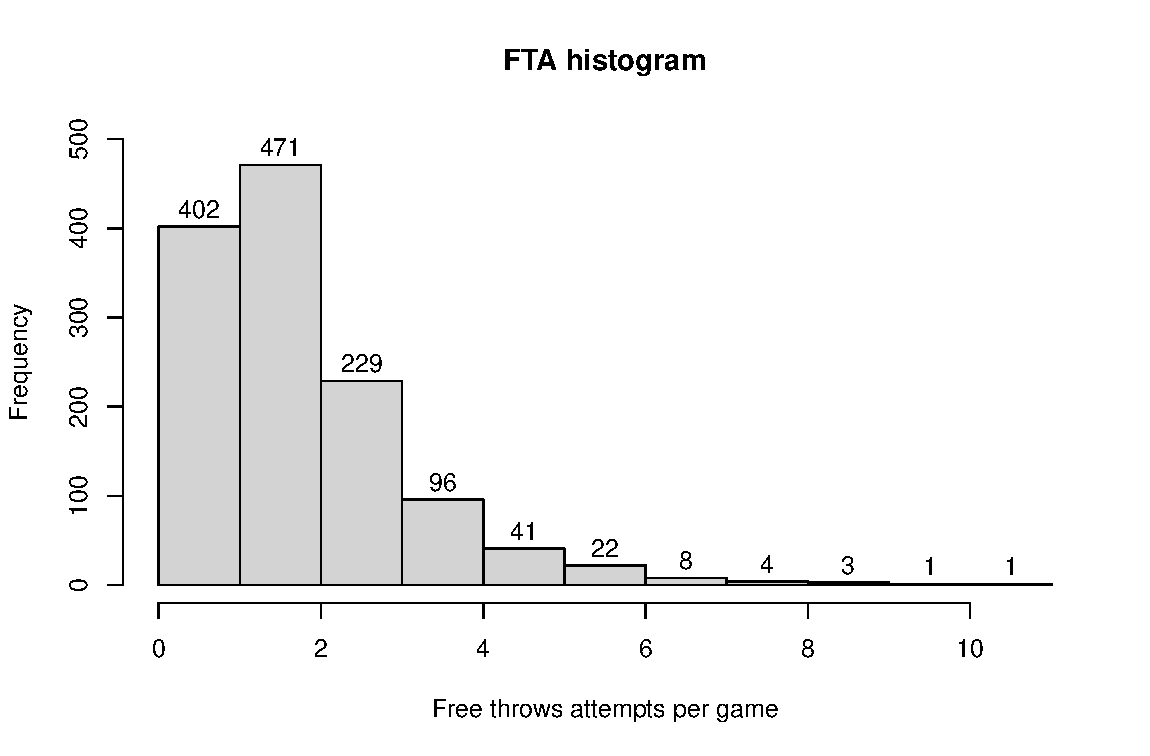
\includegraphics[width=0.5\linewidth]{ImageFiles/Histograms/histogram_fta}
		\caption{}
		\label{fig:HistFTA}
	\end{subfigure}%
	\begin{subfigure}{.3\textwidth}
		\centering
		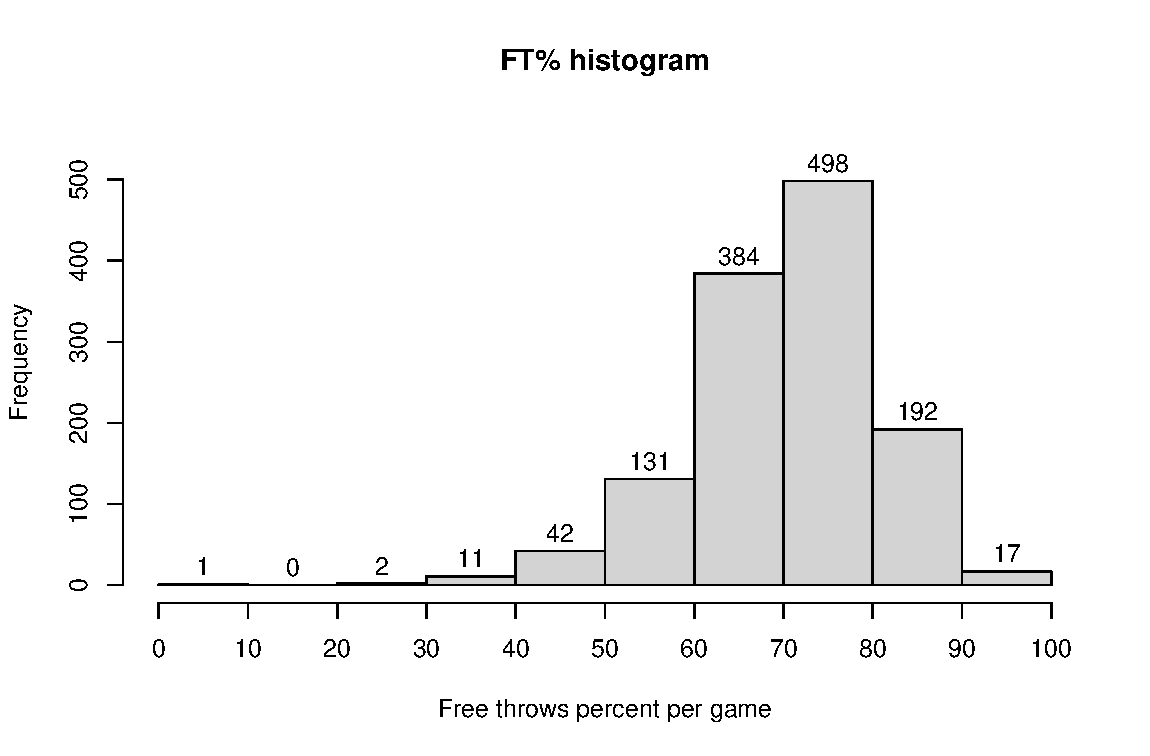
\includegraphics[width=0.5\linewidth]{ImageFiles/Histograms/histogram_ft}
		\caption{}
		\label{fig:HistFT}
	\end{subfigure}
	\begin{subfigure}{.3\textwidth}
		\centering
		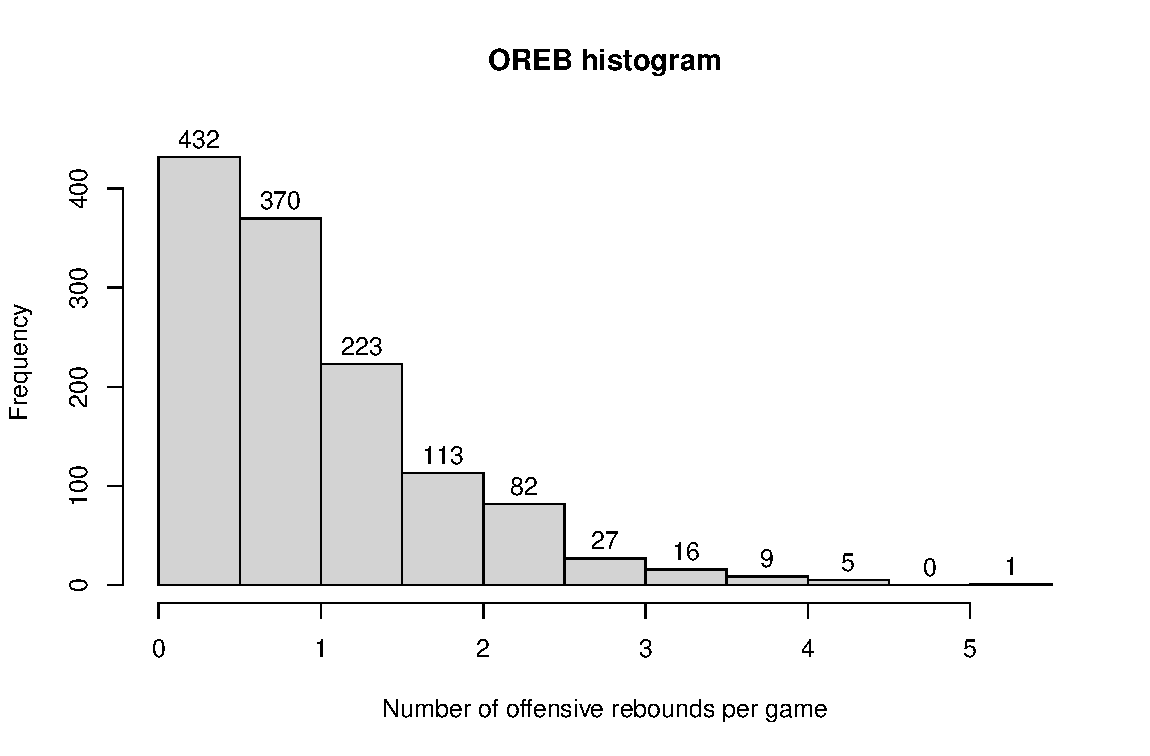
\includegraphics[width=0.5\linewidth]{ImageFiles/Histograms/histogram_oreb}
		\caption{}
		\label{fig:HistOREB}
	\end{subfigure}%
	\begin{subfigure}{.3\textwidth}
		\centering
		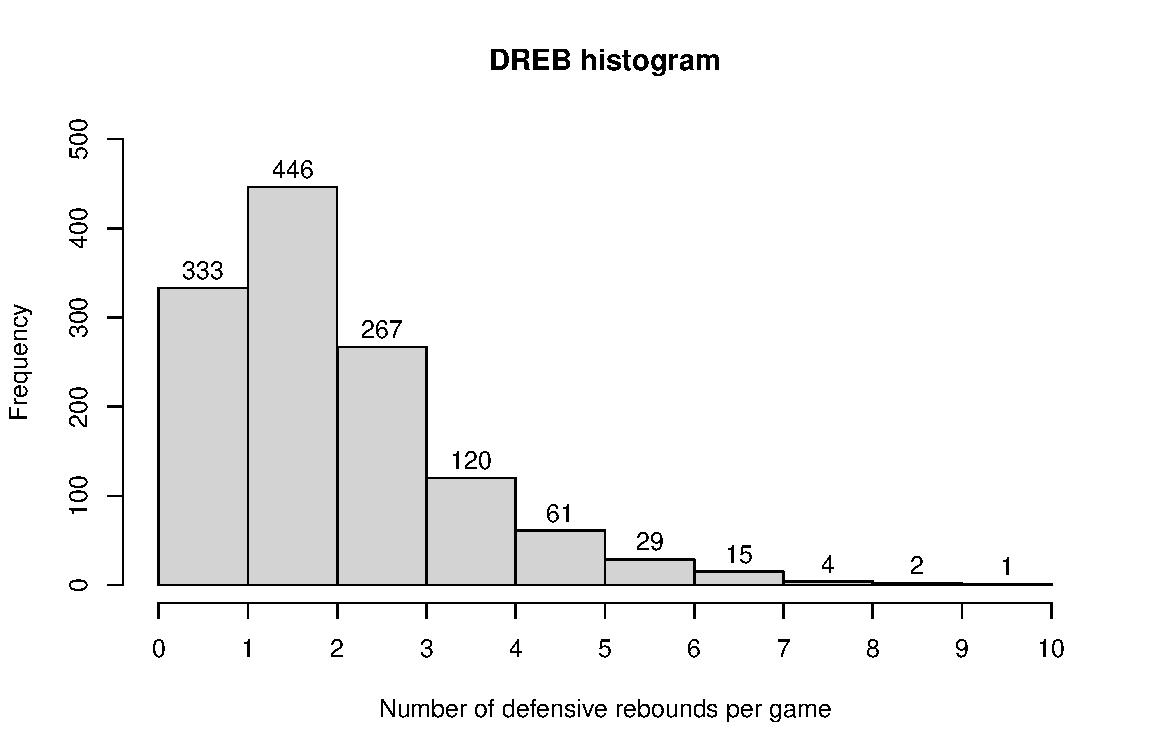
\includegraphics[width=0.5\linewidth]{ImageFiles/Histograms/histogram_dreb}
		\caption{}
		\label{fig:HistDREB}
	\end{subfigure}%
	\begin{subfigure}{.3\textwidth}
		\centering
		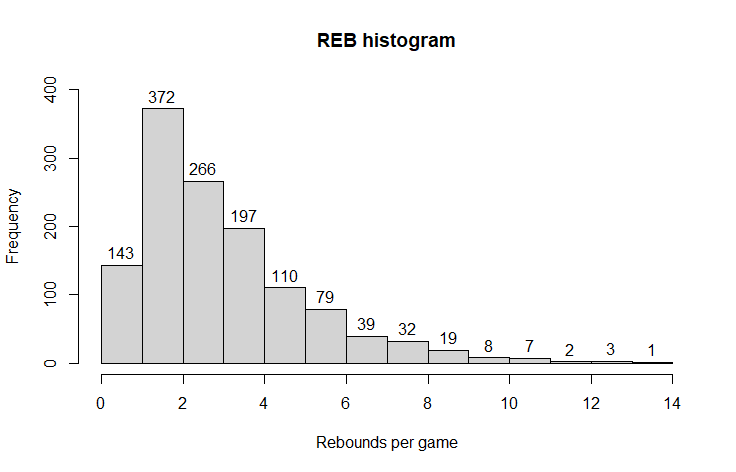
\includegraphics[width=0.5\linewidth]{ImageFiles/Histograms/histogram_reb}
		\caption{}
		\label{fig:HistREB}
	\end{subfigure}
	\begin{subfigure}{.3\textwidth}
		\centering
		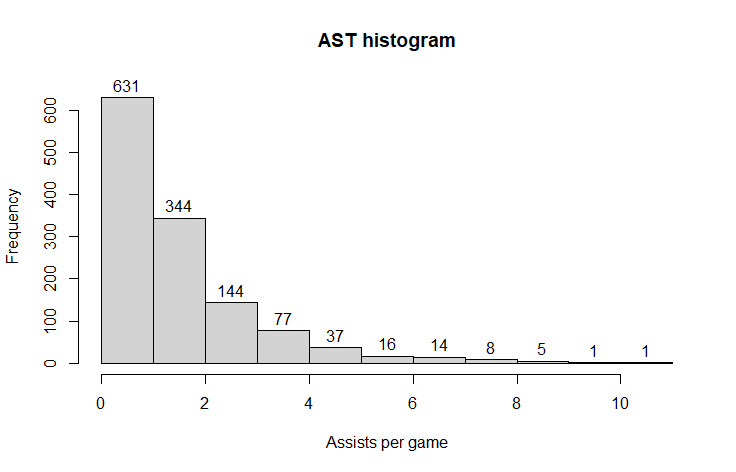
\includegraphics[width=0.5\linewidth]{ImageFiles/Histograms/histogram_ast}
		\caption{}
		\label{fig:HistAST}
	\end{subfigure}%
	\begin{subfigure}{.3\textwidth}
		\centering
		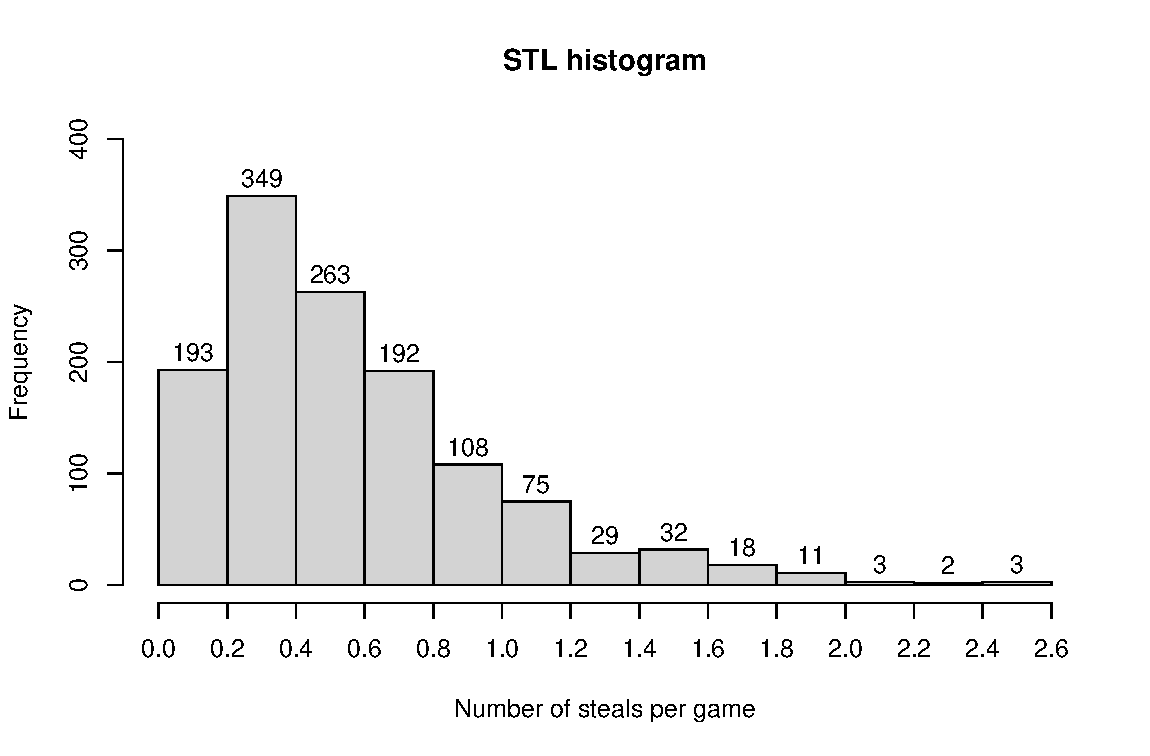
\includegraphics[width=0.5\linewidth]{ImageFiles/Histograms/histogram_stl}
		\caption{}
		\label{fig:HistSTL}
	\end{subfigure}%
	\begin{subfigure}{.3\textwidth}
		\centering
		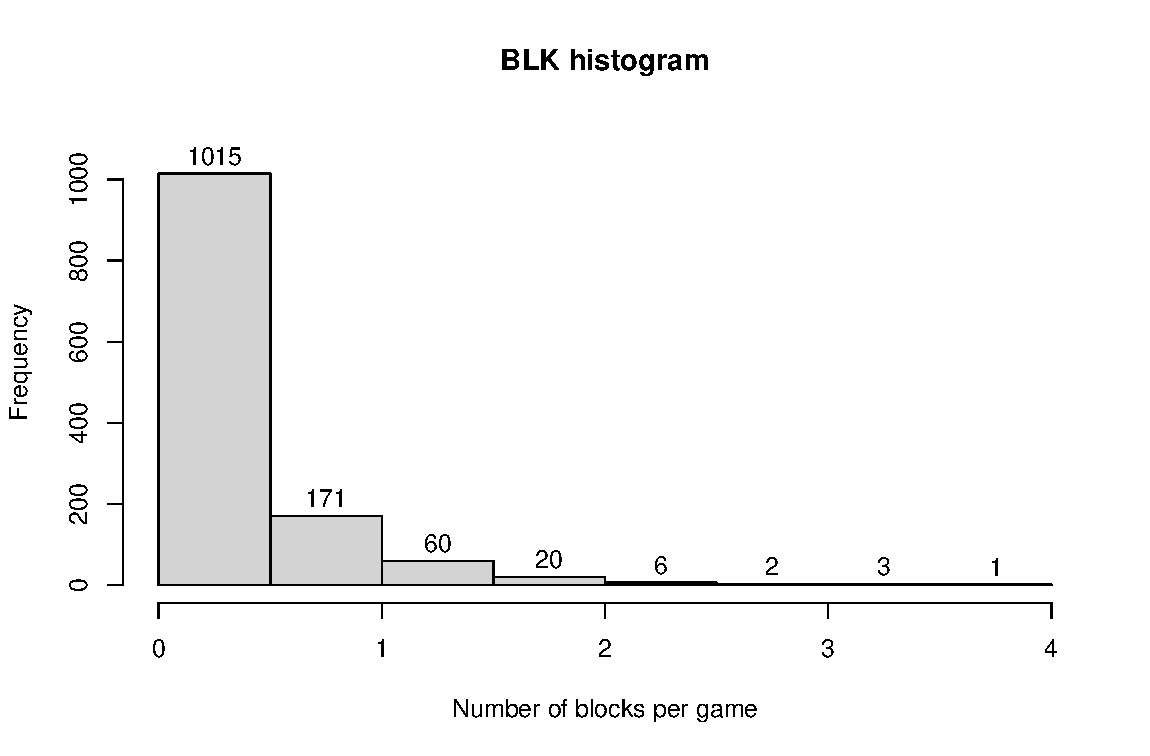
\includegraphics[width=0.5\linewidth]{ImageFiles/Histograms/histogram_blk}
		\caption{}
		\label{fig:HistBLK}
	\end{subfigure}
	\begin{subfigure}{.3\textwidth}
		\centering
		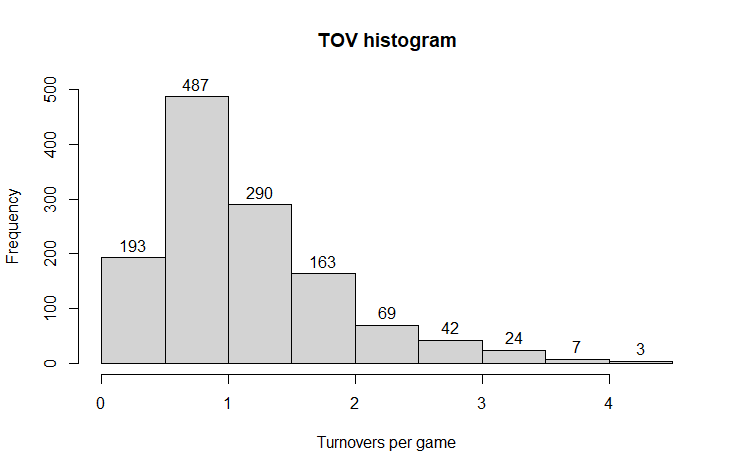
\includegraphics[width=0.5\linewidth]{ImageFiles/Histograms/histogram_tov}
		\caption{}
		\label{fig:HistTOV}
	\end{subfigure}
	\caption{Variable histograms.}
	\label{fig:Histograms}
\end{figure}

We can also look at the output variable to check whether the dataset was balanced or not. In \Fig~\ref{fig:target_bar_plot} we can clearly see that the samples are not equally distributed. 

\begin{figure}[H]
	\centering
	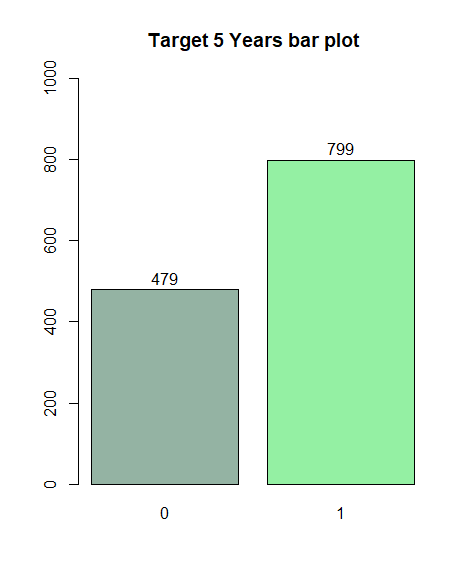
\includegraphics[width=0.5\linewidth]{ImageFiles/Histograms/target_bar_plot}
	\caption{Target variable bar plot.}
	\label{fig:target_bar_plot}
\end{figure}

%Besides ``Name, ``GP'' and ``TARGET\_5Yrs'', each feature is intended to be expressed ``per game''.
The objective of this analysis is to develop two distinct models that can effectively explain the features ``PTS'' and ``TARGET\_5Yrs''. Due to the nature of these variables, two different approaches are required. For ``PTS'', a regression method must be utilized due to its continuous nature, whereas for ``TARGET\_5Yrs'', a classification method must be employed given that it is a binary variable.